\setchapterpreamble[u]
{%
	\renewcommand*{\dictumrule}{\par}
	\let\dictumwidth\textwidth
	\dictum{\normalfont\itshape\raggedleft Translated by George Balabanian}
	\bigskip\par
}


\chapter{Translation of Adjarian 1899 on voice onset time}\label{chapter:George}

	
	\translatorHD{Below is a translation of \citet{Adjarian-1899-ArmenianExplosives}, done by George Balabanian. That paper is an early acoustic demonstration of voice onset time, using Armenian data \citep{braun-2013-earlyCaseVOTAdjarian}. } 

\textbf{Original title:} Les Explosives de l'ancien arménien étudiées dans les dialectes modernes

\textbf{Translated title:} The stops and affricates of Classical Armenian, studied in modern dialects

\section{Introduction, background, and methodology}




Here, I investigate what has become of the three groups of Classical Armenian stops and affricates in the modern dialects.

\translatorHD{The French term that Adjarian uses is ``explosives,'' which is no longer used today. It was generally used in the 19th century to describe stops (plosives), and sometimes both stops and affricates (which is the way Adjarian uses it). The term `obstruent' is too wide a term, as it would include all fricatives, stridents, and sibilants. And `occlusive' is also too wide, as it also includes nasals.}



\begin{table}[H]
	\resizebox{\textwidth}{!}{%
	\begin{tabular}{llll}
			\lsptoprule Adjarian's original  & Armenian  & IPA transcription & Hübschmann-Meillet  \\
			notation & orthography &     &     transliteration \\
			 \cmidrule(lr){1-1}  \cmidrule(lr){2-2}        \cmidrule(lr){3-3}  \cmidrule(lr){4-4}      
			b, g, d, dz, dj & \armenian{բ, գ, դ, ձ,   ջ} & b, g, d, d͡z, d͡ʒ & b, ɡ, d, j, ǰ   \\
			p, k, t, ts, tch & \armenian{պ, կ, տ, ծ,   ճ} & p, k, t, t͡s, t͡ʃ & p, k, t, c, č  \\
			pᶜ, kᶜ, tᶜ, tsᶜ,   tchᶜ & \armenian{փ, ք, թ, ց,   չ} & pʰ, kʰ, tʰ,   t͡sʰ, t͡ʃʰ & pʿ, kʿ, tʿ, cʿ, čʿ  
			\\ \lspbottomrule 
		\end{tabular}
}
\end{table}


I limit my study only to word-initial sounds and to differences in sonority and intensity.

The sonority of a consonant is determined by the relationship between two moments: the moment when the consonant bursts out by the effect of the air being expelled from the mouth, and the moment when the larynx vibrates. The intensity is proportional to the amount of air expended for the explosion. To determine these various data, I used the experimental method. In other words, I had recourse to the phonetic laboratory and machines of the Abbot Rousselot.\footnote{Jean-Pierre Rousselot (1846-1924) was a French priest and is considered the founder of experimental phonetics.}

I collected the movements of the speech air column with a mouthpiece, and the vibrations of the larynx with a capsule attached to the thyroid cartilage with a rubber tie. Both phenomena were recorded on a rotating cylinder by means of two lever drums mounted to capture the vibratory movements and acting simultaneously.

Each of my plots thus consists of two synchronic lines: the top one marking the air displacement, or speech, the lower one, laryngeal vibrations.

I've indicated synchronicity by means of vertical construction lines. The dotted lines indicate when the larynx begins to vibrate; solid lines indicate the moment of burst.

All plots are comparable in terms of sound sonority. But for the various degrees of intensity, it is only legitimate to compare between plots relating to the same dialect, as my experiments were carried out at rather different times and with different equipment.



\translatorHD{Adjarian listed data from the following dialects, along with an abbreviation:}

\begin{itemize}
	\item C = Constantinople; 1 2 3 mark three variants of popular pronunciation: C1 emphatic pronunciation, C2 normal pronunciation, C3 exceptional pronunciation.
	
	\translatorHD{See the Istanbul chapter \S\ref{section:istanbul:phono:inventory:cons} and \S\ref{sec:Istanbul:phono:soundchange:cons:laryngeal}.}
	\item A = Aslanbeg 
	
	
	\translatorHD{The Aslanbeg variety is a subdialect of the Nicomedia dialect. See \S\ref{section:nicomedia:phono:inventory}.}
	\item N = Nukha
	
	\translatorHD{French spelling is Nouxa; also spelled Nukhi, Nukha; Shaki (Şəki) of modern-day Azerbaijan, \armenian{Նուխի} or \armenian{Շաքի} in Armenian, part of the Karabakh/Artsakh dialect group. For general information on the consonant system of Karabakh, see \S\ref{section:karabakh:phono:inventory:cons} and \S\ref{section:karabakh:phono:change:cons}.} 
	\item M = Mush: M1 first category of voiced consonants; M2 second category of voiced consonants.
	
	\translatorHD{For more information on Mush, see \ref{section:mush:phono:change:cons}.}
	\item Ch  = Shushi
	
	\translatorHD{Originally \textit{Ch} for \textit{Choucha} (Shushi, Shusha).} 
	
	\translatorHD{The Shushi vernacular is part of the Karabakh dialect group. For general information on the consonant system of Karabakh, see \S\ref{section:karabakh:phono:inventory:cons} and \S\ref{section:karabakh:phono:change:cons}.}
	\item S = Sivas
	
	\translatorHD{Also commonly known as Sebastia.}
	
	\translatorHD{For more information on Sebastia, see \S\ref{section:sebastia:phono:inventory:cons}.} 
	
	
\end{itemize}

 

\begin{figure}
	\centering
	\resizebox{\textwidth}{!}{%
	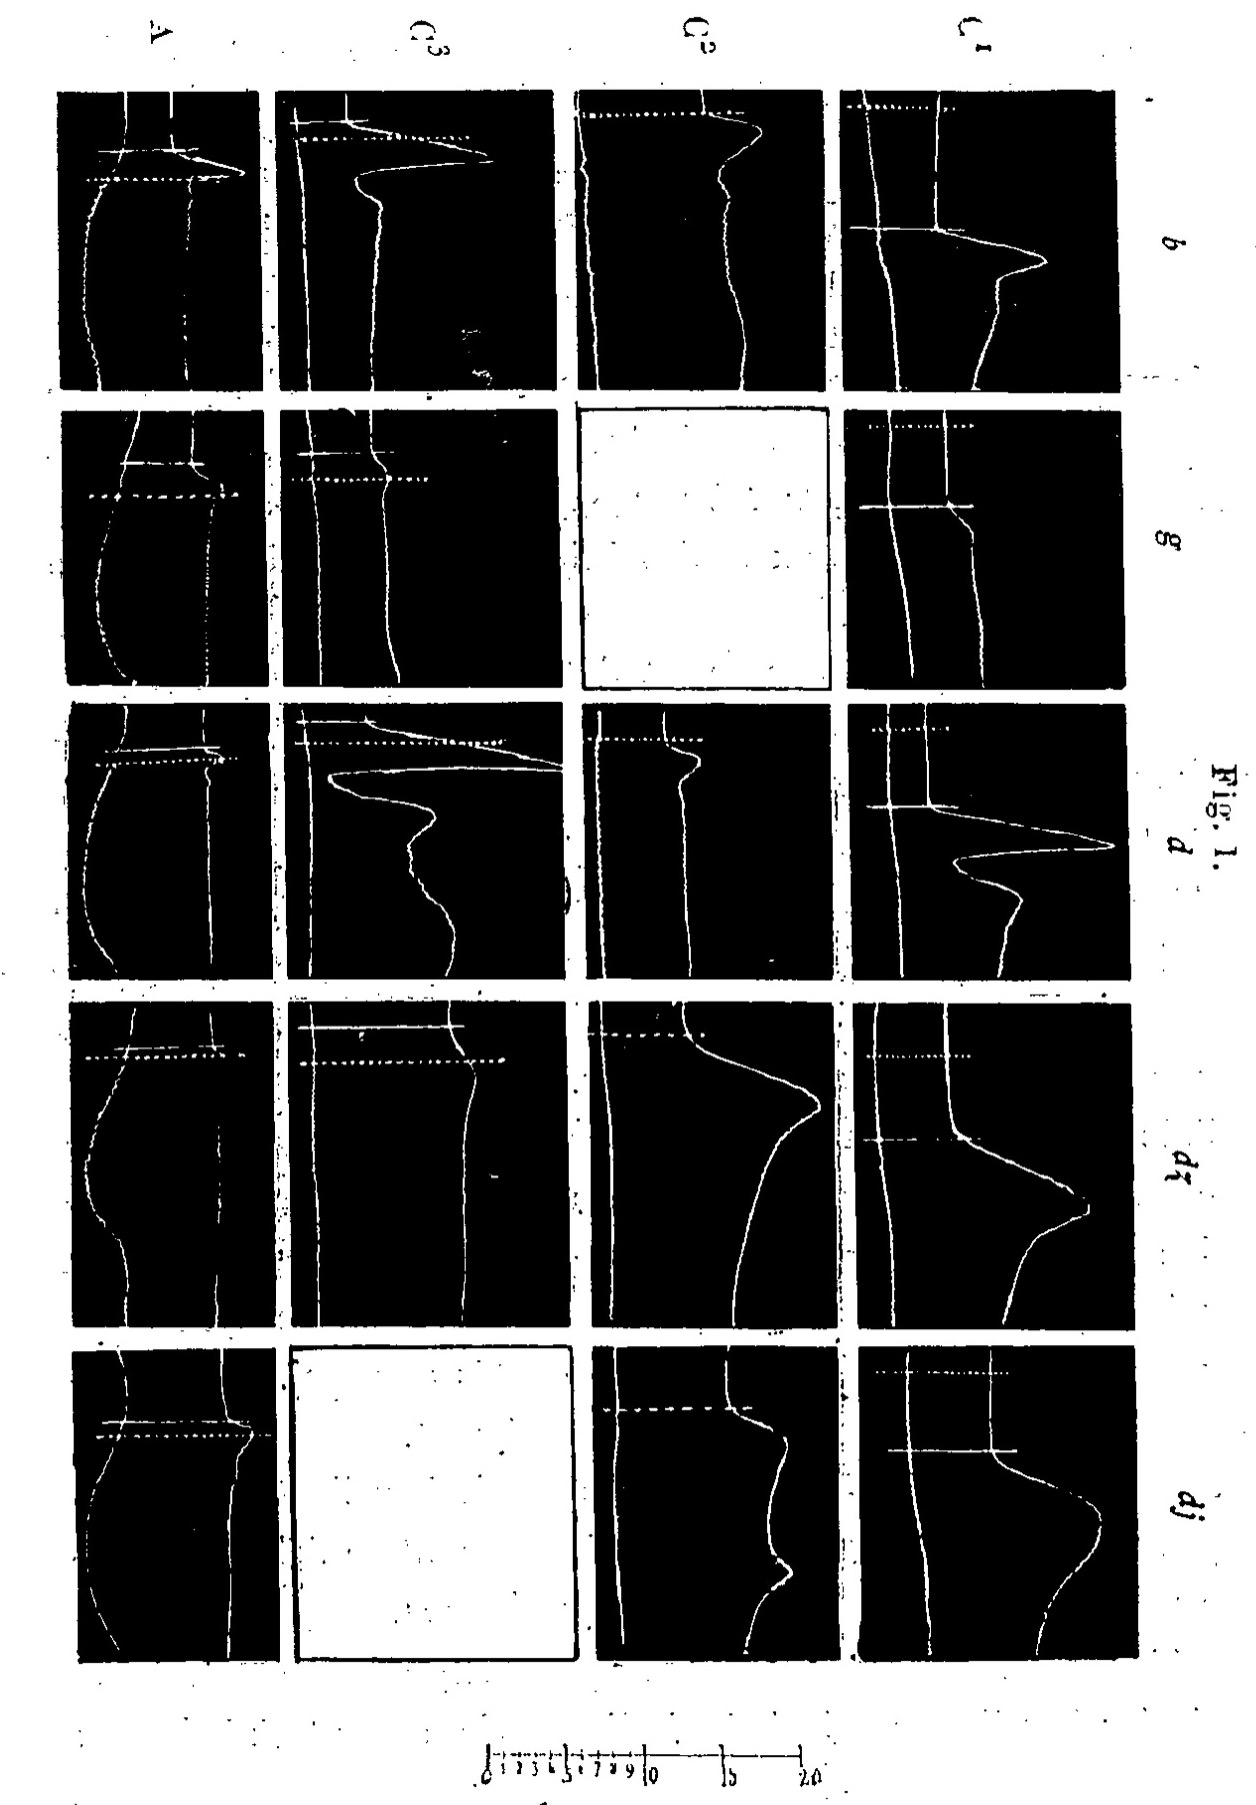
\includegraphics[scale= .3]{images/adjarian1899fig1.jpg}
}
	\caption{Original figure 1 for reflexes of Classical Armenian voiced stops and affricates}
	\label{fig:fig1 original}
\end{figure}

\begin{figure}
	\centering
	\resizebox{\textwidth}{!}{%
	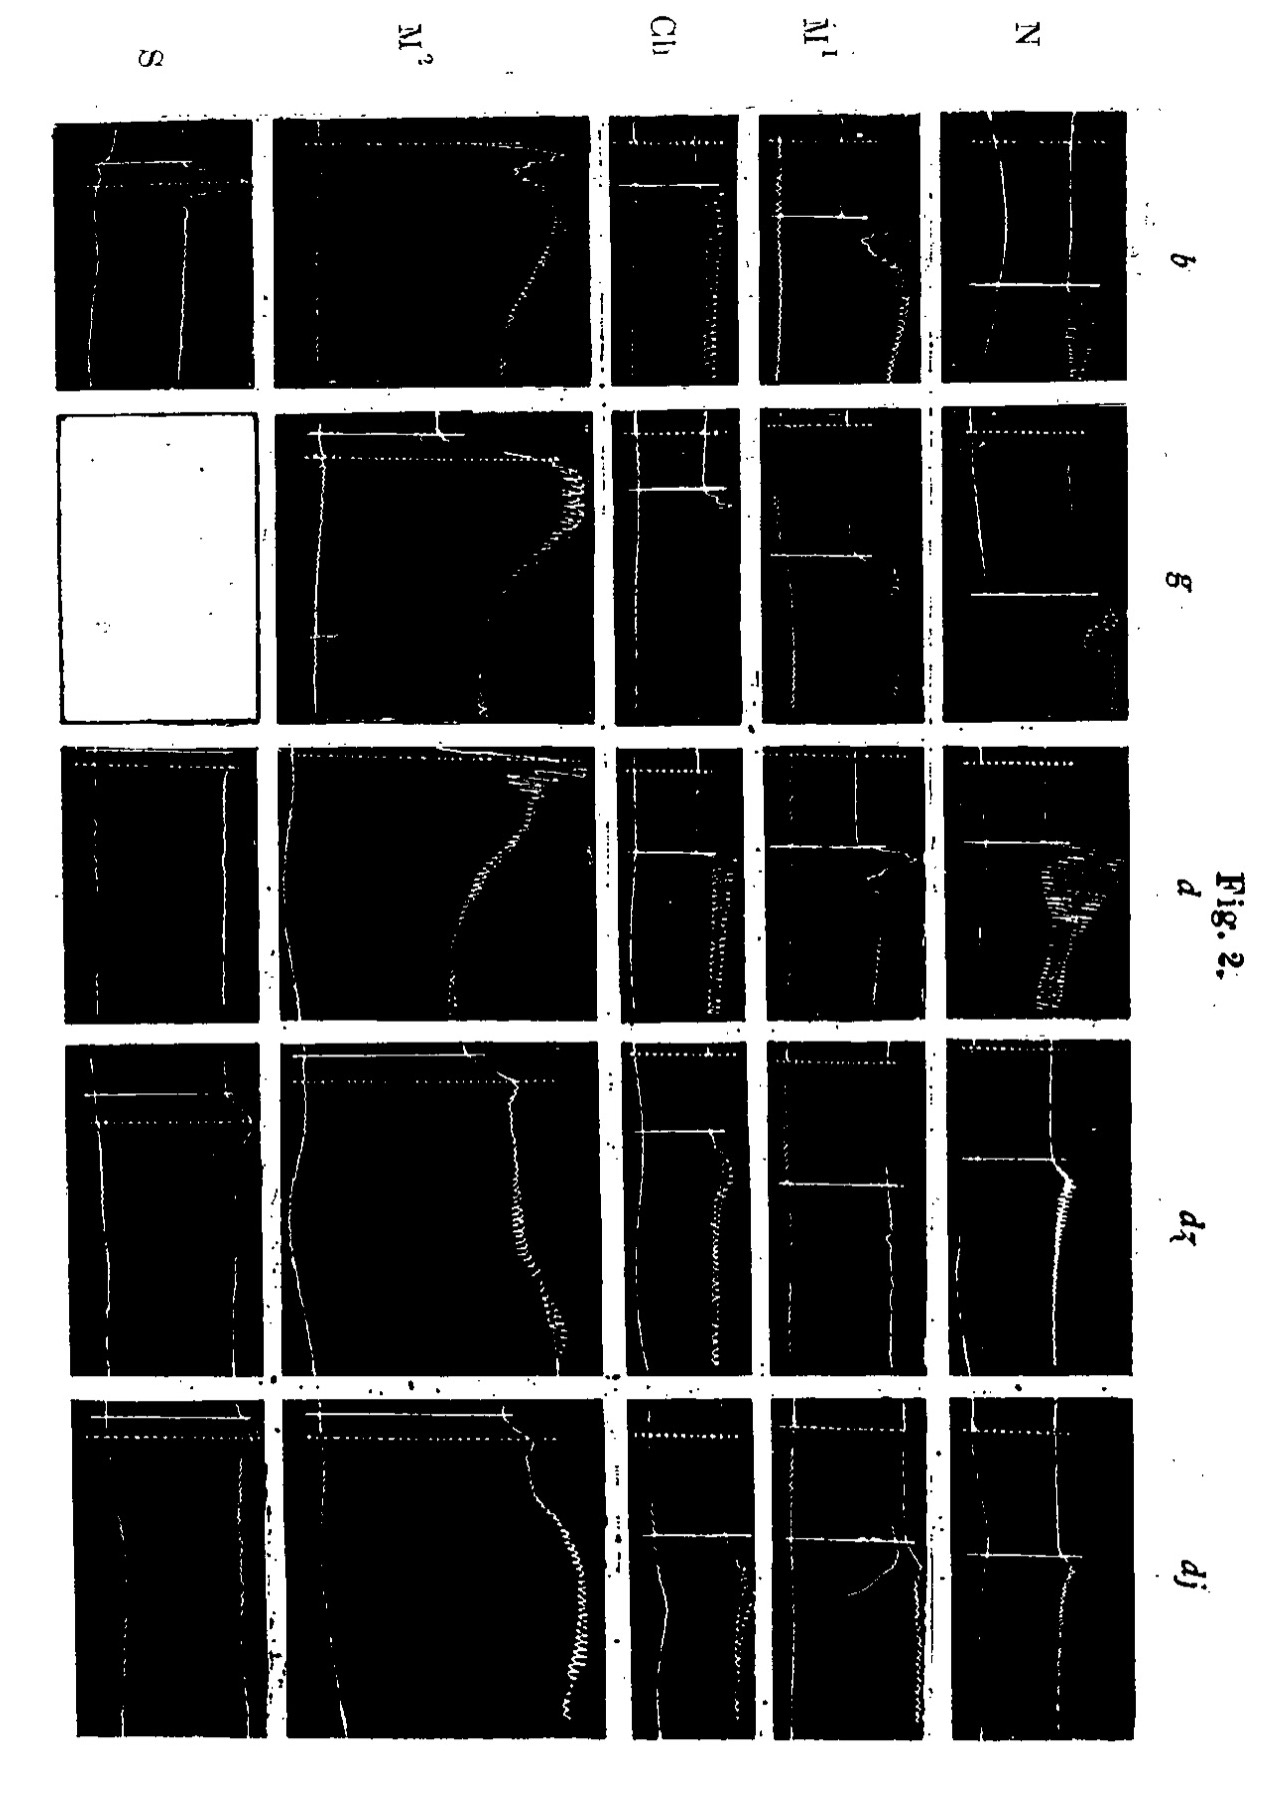
\includegraphics[scale= .3]{images/adjarian1899fig2.jpg}
}
	\caption{Original figure 2 for reflexes of Classical Armenian voiced stops and affricates}
	\label{fig:fig2 original}
\end{figure}


\begin{figure}
	\centering
	\resizebox{\textwidth}{!}{%
	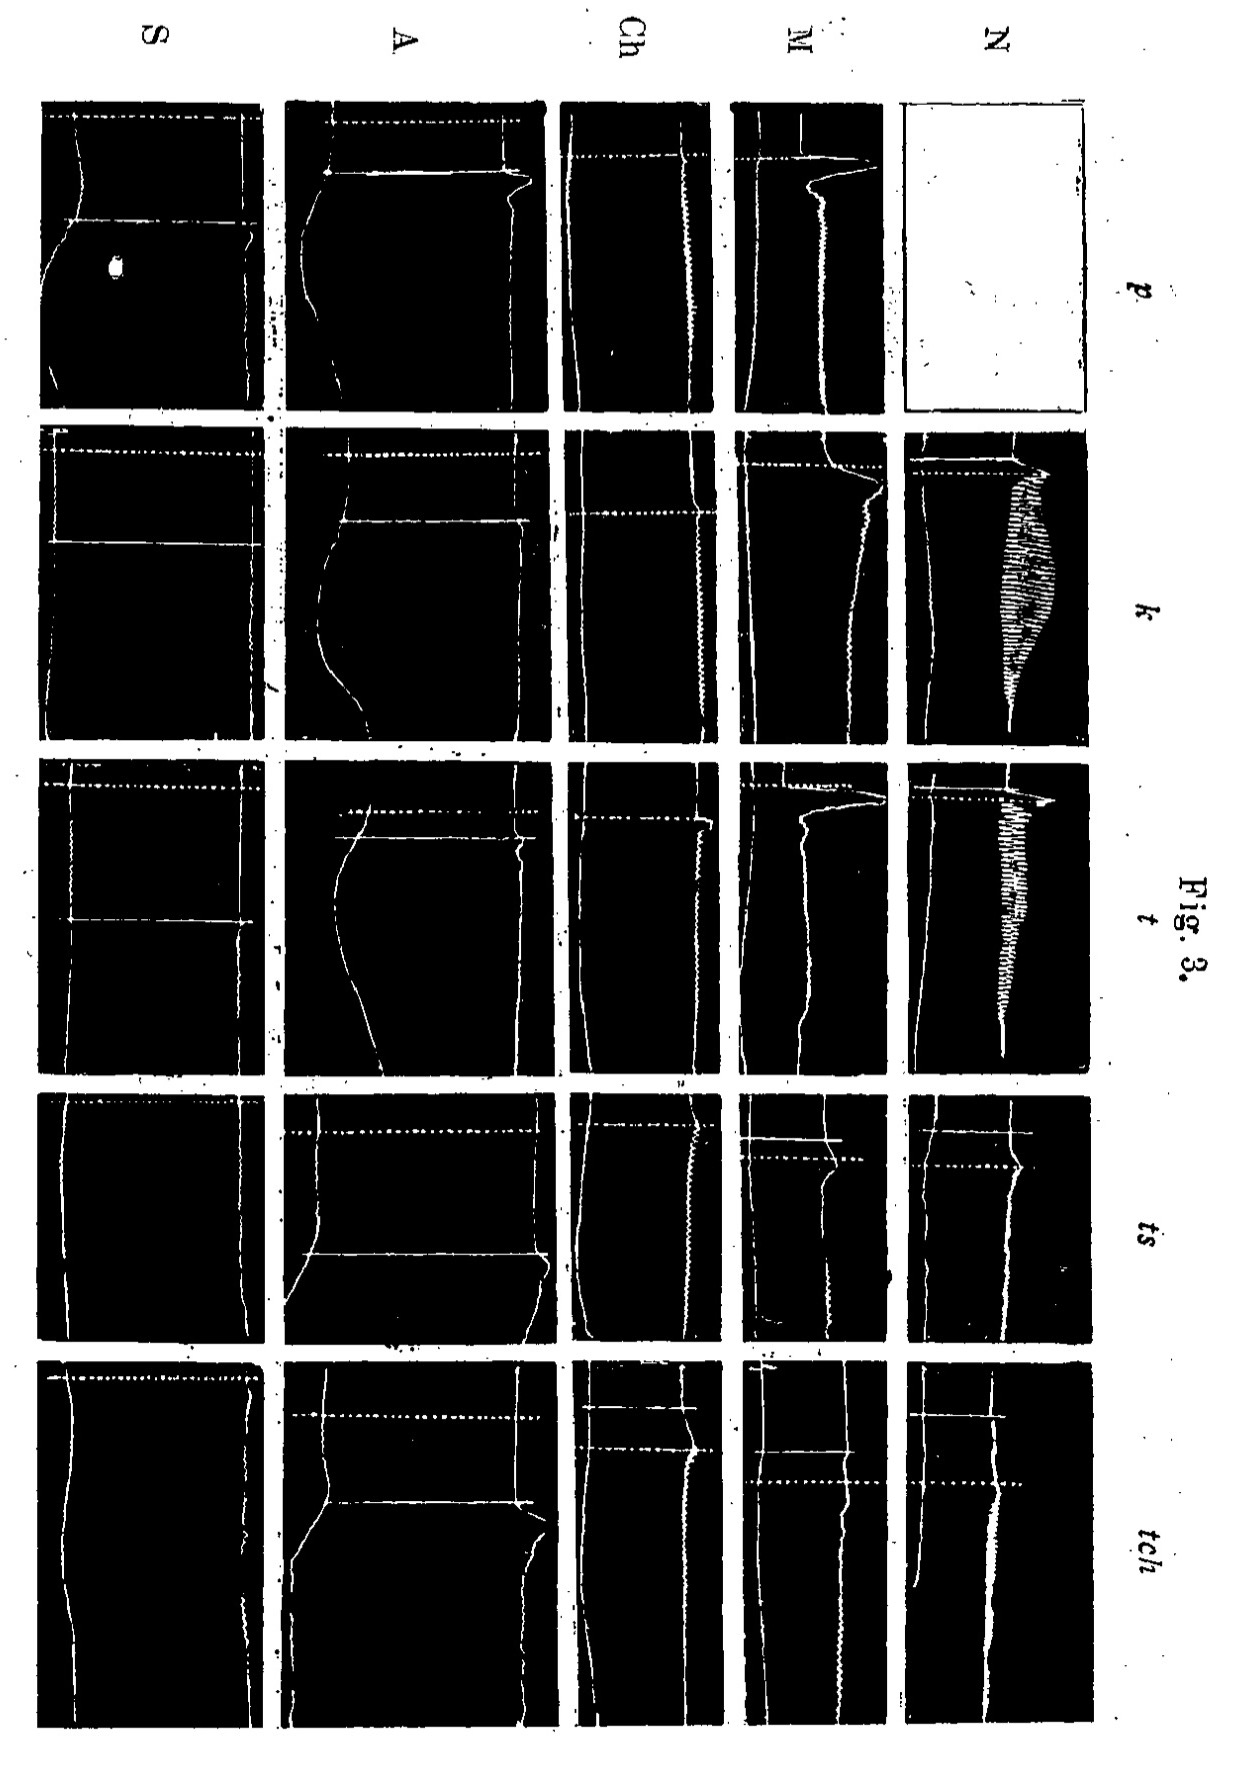
\includegraphics[scale= .3]{images/adjarian1899fig3.jpg}
}
	\caption{Original figure 3 for reflexes of Classical Armenian voiceless unaspirated stops and affricates}
	\label{fig:fig3 original}
\end{figure}


\begin{figure}
	\centering
	\resizebox{\textwidth}{!}{%
	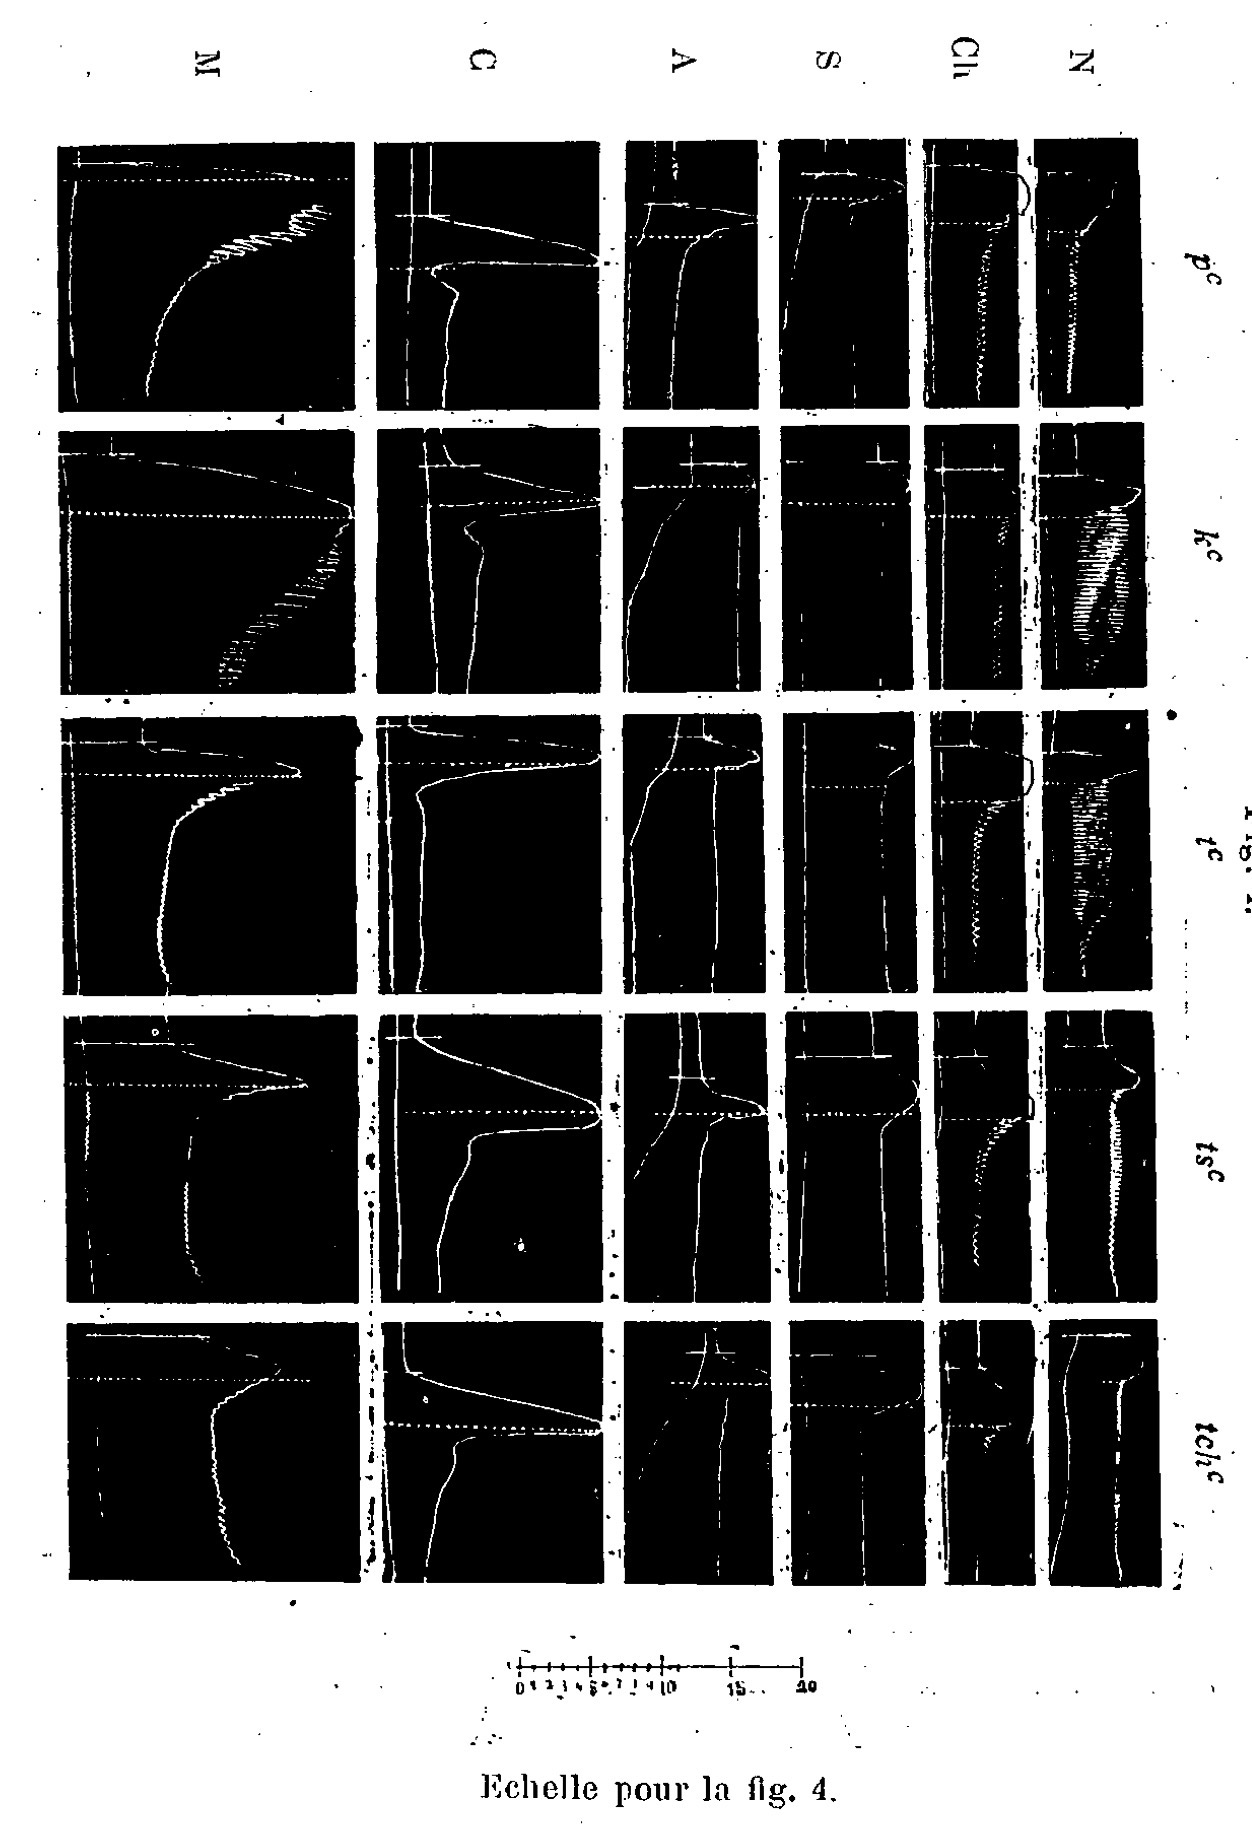
\includegraphics[scale= .3]{images/adjarian1899fig4.jpg}
}
	\caption{Original figure 4 for reflexes of Classical Armenian voiceless aspirated stops and affricates}
	\label{fig:fig4 original}
\end{figure}



One would be struck, I'm sure, by the amplitude of some of the vibrations, or the apparent weakness of some of the bursts. It's important not to dwell on this: it is all due, not to the phenomenon itself, but to the nature of the drum I have used.

To make it easier to compare my plots, I've grouped them in four tables, arranged so that the same articulation is read from top to bottom, and that the forms of the same dialect follow each other horizontally. When an articulation is missing in a dialect, the place it should occupy is left blank.

Two scales are used to measure the duration in hundredths of a second. The first, appended to Figure \ref{fig:fig1 original}, is used for tables 1, 2 and 3 ; the 2nd, for Figure \ref{fig:fig4 original}, to which it is attached.

The figures have been reproduced by photogravure. Some have been edited, but only for points that are outside the purpose of this work.

The experiments were carried out on the following people, each using the speech of his native town:

\begin{enumerate}
	\item First, myself, Hratchia Adjarian, born in 1874, in Constantinople (250,000 Armenians), for the popular and literary pronunciations.
	\item Mr. Alexandre Nalbandian, born in 1873, in Aslanbeg, a large Armenian village (4,000 inhabitants) near the town of İzmit (Ismidt), on the Sea of Marmara.
	
	\item Mr. Vahan Ter-Poghossian, born in 1872 in Nukha, on the southern side of the Caucasus, east of Tbilisi (Tiflis.
	
	\item The melik Nikoghos Avcharian, born in Shushi, in 1872.
	
	\item Mr. Tigran Dimaksian, born in 1878, in Karmen, an Armenian village near Mush.
	
	\item Mr. Georg Mkrtichian, born in Sivas in 1872.
	
\end{enumerate}


\section{The voiced stops and affricates of Classical Armenian}

\armenian{բ, գ, դ, ձ, ջ} – /b, ɡ, d,  d͡z,  d͡ʒ/ (Figures \ref{fig:fig1 original} and \ref{fig:fig2 original})... 

1. In the popular speech of Constantinople (C1, C2, C3), there are three ways of pronouncing these consonants: for the first manner, the laryngeal vibrations precede the air burst (by 0.08 seconds): for the second manner, the laryngeal vibrations occur at the same time as the air burst, and for the third manner, the vibrations occur slightly after the air burst (by only 0.01-0.02 seconds).

So, in reality, we have 3 varieties of voiced stops and affricates (3 \textit{b}, 3 \textit{ɡ}, 3 \textit{d}, etc.), but the third is far less distant from the second than this one is from the first.

The first, which corresponds exactly to French voiced consonants, is used when there is emphasis; it can therefore be called emphatic. The second, which corresponds to German voiced consonants, can be called normal, as the vast majority of examples belong to this type: such is the ordinary pronunciation of Constantinople. As for the third, I have only observed it accidentally. These voiced consonants are close to the corresponding voiceless ones, but they have less force, and the larynx enters into vibration faster than for the voiceless consonants.

2. In the literary language of Constantinople and in the dialect of Aslanbeg (A), voiced consonants are pronounced voiceless aspired consonants, which we'll discuss later (Figure \ref{fig:fig4 original} C, and A). However, in Aslanbeg, these consonants have less force than the corresponding aspirated ones (compare Figure \ref{fig:fig1 original}A and \ref{fig:fig4 original}A). Occasionally, they are pronounced like the voiced ones in the popular Constantinople speech (Figure \ref{fig:fig1 original} C1, C2, C3).

3. In the dialects of Nukha (N) and Shushi (Ch), they have remained completely voiced; vibrations of the larynx begin at variable times, up to more than 0.1 of a second before the air burst.

4. In the dialects of Mush (M1 M2) and Sivas (S), they have two distinct categories. The first (M1) presents voiced consonants in Nukha and Shushi. In the second (M2 and S), the consonant is pronounced more strongly than in the first, and the volume of air from the burst is more considerable,  which gives me the impression of a <bh> or a voiced [b] ([bʰ]) followed by a confused noise in the throat, whereas a French speaker hears [p].

The laryngeal vibrations begin 0.02-0.03 seconds after the air burst; but in two instances, for [b], there was simultaneity between the start of laryngeal vibrations and the air burst.

\section{The voiceless unaspirated stops and affricates of Classical Armenian}

\armenian{պ, կ, տ, ծ, ճ} – /p,  k,  t, t͡s,  t͡ʃ/
(Figure \ref{fig:fig3 original})

1. In the vernacular and literary languages of Constantinople, these consonants are considered voiced and are pronounced exactly like these (Figure \ref{fig:fig1 original} C1 C2 C3).

2. Similarly, in Aslanbeg and Sivas (A, S), they have become voiced: vibrations begin between 0.015 and 0.08 seconds before the air burst.

3. In the other dialects (N, M, Ch), they have remained voiceless, and perfectly distinct from both the corresponding voiced and voiceless aspirated consonants.

In Nukha (N) and Shushi (Ch), laryngeal vibrations begin at the moment when air emission is impeded, which corresponds to the fall of the plotline after the first moment of the air burst.

In Mush (M), laryngeal vibrations generally begin at the same time as the air burst. Nevertheless, my examples of [t͡s] and [t͡ʃ] show exactly the same position as in the pronunciation of Nukha and Shushi. I've also found the same for the consonant [t].

In Mush, unaspirated consonants can also become voiced as in the dialects of Constantinople, Sivas, and Aslanbeg.


\section{The  voiceless aspirated stops and affricates of Classical Armenian}

\armenian{փ, ք, թ, ց, չ} –  pʰ, kʰ, tʰ,  t͡sʰ,  t͡ʃʰ


In Constantinople, in the popular and literary pronunciations, these are divided into 3 classes. In the first, the vibrations of the larynx occur 0.01 second after the start of the air burst; this corresponds roughly to the strong French consonants (Figure \ref{fig:fig1 original} C3). In the second case, vibrations begin at the point where air emission is hindered, in other words, at the highest point of the plotline (Figure \ref{fig:fig4 original} C, except for [pʰ]). In the third case, vibrations occur after the movement of airflow, or very shortly before (Figure \ref{fig:fig4 original} C, [pʰ]). But the first and third classes are very rare; I have merely found them accidentally.

2. In Mush (M), the situation is similar to the second class described for Constantinople.

3. In the other dialects (N, Ch, S, A), these consonants are completely voiceless: vibrations only begin after the air burst is completed.
	
	
